\chapter{Data}
\label{Da}

This study uses daily financial data of all the constituents of the Oslo Stock Exchange All-Share Index (OSEAX), obtained from Factset, between January 2010 and September 2017. Stocks that are not continuously listed during the period is excluded. In addition, we have excluded stocks following the criterion employed by Fu \cite{Fu}, which requires that each stock must be traded for a minimum of 15 days during each month of the sample period. The number of constituents in the index is 168 before cleaning and 105 after cleaning. This paper is based on the cleaned data. For the selected stocks, after data cleaning, we refer to appendix B. 

All the financial data is retrieved from FactSet. In addition to the Norwegian 10-years government bonds daily closing prices, we retrieved the following data for each stock:
\begin{itemize}
    \item Closing price, daily
    \item Total shares outstanding, daily
    \item Book value, rolling last twelve month
\end{itemize}

In the upper part of Figure \ref{MarketReturn} the economic return of the equally weighted portfolio containing the selected stocks is visualized. This portfolio will be referred to as the market portfolio and is rebalanced daily. The portfolio has a return of $106\%$ from January 2010 to September 2017. In addition, we show the squared daily economic return in bottom part of Figure \ref{MarketReturn}. We observe volatility clustering in the squared daily economic returns, suggesting that non-linear effects are present.

\begin{figure}[h]
\label{MarketReturn}
    \centering
    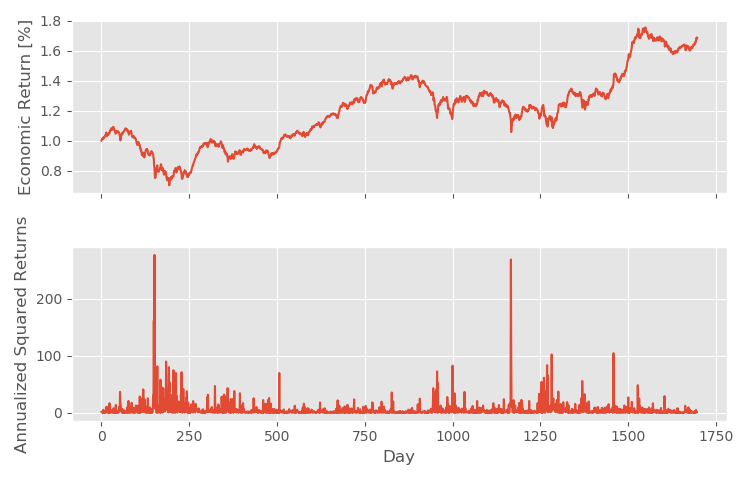
\includegraphics[scale = 0.7]{Plot/MarketReturn.png}
    \caption{Economic Return of the Equally Weighted Market Portfolio}
    \label{MarketReturn}
\end{figure}

In Table \ref{DesStat} we present the descriptive statistics of the daily economic return distribution of the market portfolio. We observe that the market portfolio has a positive daily expected return of $0.04\%$. The data exhibits positive excess kurtosis, suggesting that our return distribution is a leptokurtic density. A leptokurtic density is one that has higher peak than a normal density. More peak than normal means that a distribution also has fatter tails and that there are more chances of extreme outcomes compared to a normal distribution. Moreover, the negative skew indicates that the right tail has more probability density than the left tail. As a result, the mean is being skewed to the left of the center of the data. This is verified in Figure \ref{PercentilePlot} and Figure \ref{QQPlot}, as we observe that the economic return distribution is closely related, but not equal to a normal distribution.  

\begin{figure}
\centering
\begin{minipage}{.5\textwidth}
  \centering
  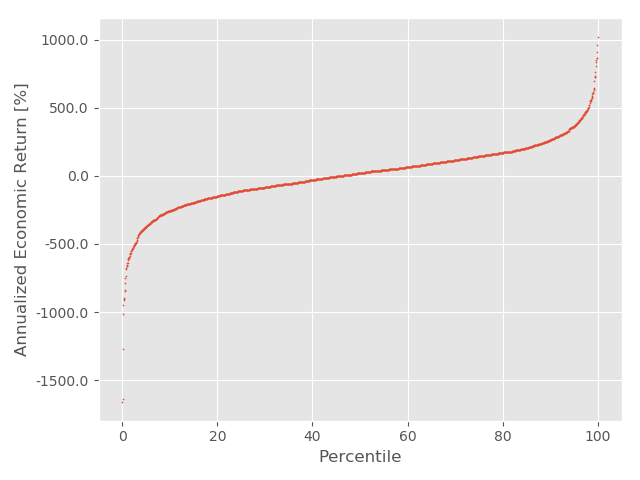
\includegraphics[scale=0.5]{Plot/PercentilePlot.png}
  \captionof{figure}{Percentile Plot}
  \label{PercentilePlot}
\end{minipage}%
\begin{minipage}{.5\textwidth}
  \centering
  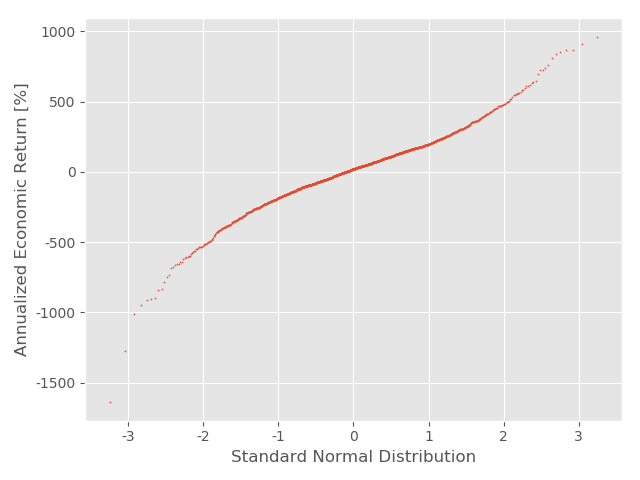
\includegraphics[scale=0.5]{Plot/QQPlot.png}
  \captionof{figure}{QQ Plot}
  \label{QQPlot}
\end{minipage}
\end{figure}
\newcolumntype{P}[1]{>{\centering\arraybackslash}p{#1}}
%\begin{landscape}
\begin{longtable}{P{1cm}P{1.5cm}P{1.5cm}P{2.2cm}P{1.6cm}P{1.8cm}P{1.8cm}P{1cm}P{1cm}} 
\caption{Descriptive Statistics of the Equally Weighted Market Portfolio}
\label{DesStat}\\
\hline
\textbf{Obs} & \textbf{Min} & \textbf{Max}&$\boldsymbol{E[r_{economic}]}$&\textbf{Median} &$\boldsymbol{\sigma^2_{economic}}$ &$\boldsymbol{\sigma_{economic}}$ & \textbf{Skew} & \textbf{Kurt} \\
\hline
\endfirsthead
\multicolumn{9}{c}%
{\tablename\ \thetable\ -- \textit{Continued from previous page}} \\
\hline
\textbf{Max}&$\boldsymbol{E(r_{economic})}$&\textbf{Median} &$\boldsymbol{\sigma^2_{economic}}$ &$\boldsymbol{\sigma_{economic}}$ & \textbf{Skew} & \textbf{Kurt} \\
\hline
\endhead
\hline \multicolumn{9}{r}{\textit{Continued on next page}} \\
\endfoot
\hline
\endlastfoot
\input{Input/DescriptiveStatsTable.txt}
\end{longtable}